\documentclass[11pt]{article}

\usepackage[margin=2.4cm]{geometry}
\usepackage[T1]{fontenc}
\usepackage{lmodern}
\usepackage{microtype}
\usepackage{amsmath,amssymb}
\usepackage{booktabs}
\usepackage{graphicx}
\usepackage{lineno}
\usepackage[numbers,sort&compress]{natbib}
\usepackage[colorlinks=true,allcolors=blue]{hyperref}

\graphicspath{{../supplementary_code/figures/}}
\setlength{\emergencystretch}{2em}

\title{Token identity provides a fixed routing signal for residual experts in language models}
\author{Anonymous authors\\Double-anonymized manuscript}
\date{}

\begin{document}
\maketitle
\linenumbers

\begin{abstract}
Mixture-of-experts language models usually learn routers from contextual hidden states. We test whether token identity alone can allocate a narrow residual expert capacity while a shared dense multilayer perceptron preserves contextual processing. In a matched single-seed comparison, 306.5-million-parameter dense and token-routed models were trained on 8 billion FineWeb-Edu tokens. The token-routed model reached an evaluation-stream negative log-likelihood of 2.9329, compared with 2.9482 for dense, but trained more slowly. Final checkpoints were near parity on zero-shot ARC-Easy, PIQA and HellaSwag, with word perplexity 35.20 versus 35.79 on WikiText-2. A separate learned-router diagnostic reversed its short-budget advantage over dense at a matched 1-billion-token budget. These results show that fixed token identity can allocate useful residual capacity in this setting, without establishing general superiority over dense or learned routing. Larger-scale, multi-seed validation remains necessary.
\end{abstract}

Mixture-of-experts (MoE) language models conditionally select parameters for each input. Their routers commonly score experts from contextual hidden states and use auxiliary losses or bias updates to prevent load collapse\cite{shazeer2017outrageously,fedus2022switch,jiang2024mixtral}. This design couples two questions: whether conditional capacity is useful and whether selecting that capacity requires a learned contextual decision. Separating them can clarify what expert routing contributes.

Fixed assignment is a useful counterpoint. Hash Layers showed that hashes of local token features can compete with learned routers in sparse language models\cite{roller2021hash}. Token identity is an especially austere routing signal: it cannot distinguish different uses of the same token. Yet it is stable, free of router parameters and may repeatedly expose lexical items to a consistent parameter subspace. If a shared path retains common contextual computation, such a fixed signal might still allocate useful residual capacity.

We test that possibility in a deliberately asymmetric architecture. Every token passes through a shared SwiGLU multilayer perceptron (MLP). Its token identifier selects two additional narrow experts, which receive the same contextual hidden state and add a gated residual. Thus token identity selects functions but does not replace contextual representations. The primary experiment compares this architecture with a parameter-matched dense model at 306.5 million parameters and 8 billion training tokens. We also evaluate the final checkpoints on four standard tasks and report separate 100-million-parameter controls with fixed, dense and learned contextual routing.

The token-routed model crosses the dense training curve after approximately 0.8 billion tokens and retains a small negative-log-likelihood (NLL) advantage at the final common evaluation. It is slower in the present implementation, and task accuracy differences are smaller than one reported standard error. A learned contextual router leads dense at short budget but trails it at a matched 1-billion-token budget. The evidence therefore supports a narrow conclusion---fixed token identity can allocate useful residual capacity in this setting---rather than a general ranking of routing mechanisms.

\section*{Results}

\subsection*{Token identity selects a narrow residual path}

The architecture changes only the transformer's feed-forward sublayer (Fig.~\ref{fig:architecture}). Attention remains causal grouped-query attention. For token identifier $t$ in layer $l$, a fixed table returns two experts. A seeded permutation of $t\bmod E$ determines the primary expert,
\begin{equation}
r_{l,1}(t)=\pi_l(t\bmod E),
\end{equation}
and a table constructed in token-ID order assigns the least-used expert other than the primary as the secondary route. The assignment balances the number of vocabulary entries allocated to each expert, not their frequency in the training corpus.

\begin{figure}[t]
\centering
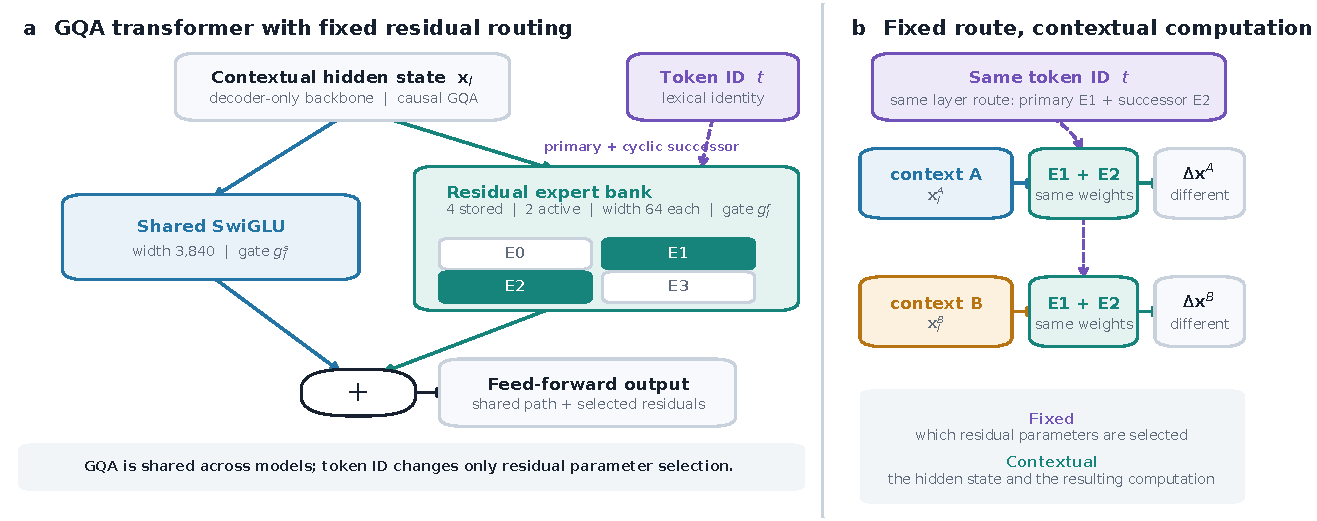
\includegraphics[width=0.98\textwidth]{architecture_complexity_deep.pdf}
\caption{\textbf{Fixed token-identity routing controls residual parameter selection.} Attention produces a contextual hidden state $\mathbf{x}$. Every token traverses the shared SwiGLU branch, while its token identifier selects two narrow residual experts through a fixed layer-specific table. All active branches transform the same contextual state; token identity is not used as an alternative representation.}
\label{fig:architecture}
\end{figure}

For contextual hidden state $\mathbf{x}$, the feed-forward output is
\begin{equation}
\operatorname{MLP}_l(\mathbf{x},t)=g_l^s\operatorname{Shared}_l(\mathbf{x})+
g_l^r\sum_{j=1}^{2}0.5\,\operatorname{Expert}_{r_{l,j}(t)}(\mathbf{x}),
\end{equation}
where $g_l^s$ and $g_l^r$ are learned scalar gates initialized to 1.0 and 0.1. Shared and routed branches are SwiGLU transformations. No auxiliary expert objective is used in the primary token-identity experiment.

The principal comparison controls the transformer backbone, tokenizer, data order, optimizer, schedule, sequence length, training-token budget and stored MLP width (Table~\ref{tab:configuration}). The routed model divides the dense width of 4,096 into a shared width of 3,840 and four stored experts of width 64. With two active experts, its evaluated MLP width per token is 3,968. Both models contain 306.5 million parameters.

\begin{table}[t]
\centering
\small
\caption{\textbf{Matched primary model configurations.} GQA, grouped-query attention. Stored routed width is $4\times64=256$; active routed width is $2\times64=128$.}
\label{tab:configuration}
\begin{tabular}{lll}
\toprule
Configuration & Token-identity residual & Dense \\
\midrule
Transformer layers & 18 & 18 \\
Model dimension & 1,024 & 1,024 \\
Attention / key--value heads & 16 / 4 (GQA) & 16 / 4 (GQA) \\
Shared MLP width & 3,840 & --- \\
Stored routed experts & 4 $\times$ 64 & --- \\
Active routed experts & 2 & --- \\
Dense MLP width & --- & 4,096 \\
Vocabulary / context & 32,000 / 2,048 & 32,000 / 2,048 \\
Total parameters & 306.5 million & 306.5 million \\
Training budget & 8 billion tokens & 8 billion tokens \\
\bottomrule
\end{tabular}
\end{table}

\subsection*{Token routing crosses dense after 0.8 billion tokens}

The routed model begins behind the dense baseline and first crosses it at the logged training point near 0.78 billion tokens (Fig.~\ref{fig:training}). Its advantage then persists through the end of training. At the last common evaluation, after 7.864 billion tokens, evaluation-stream NLL is 2.9329 for token routing and 2.9482 for dense, a difference of $-0.0153$ (Table~\ref{tab:trajectory}). Final logged training NLL is 2.9231 and 2.9324, respectively.

\begin{figure}[t]
\centering
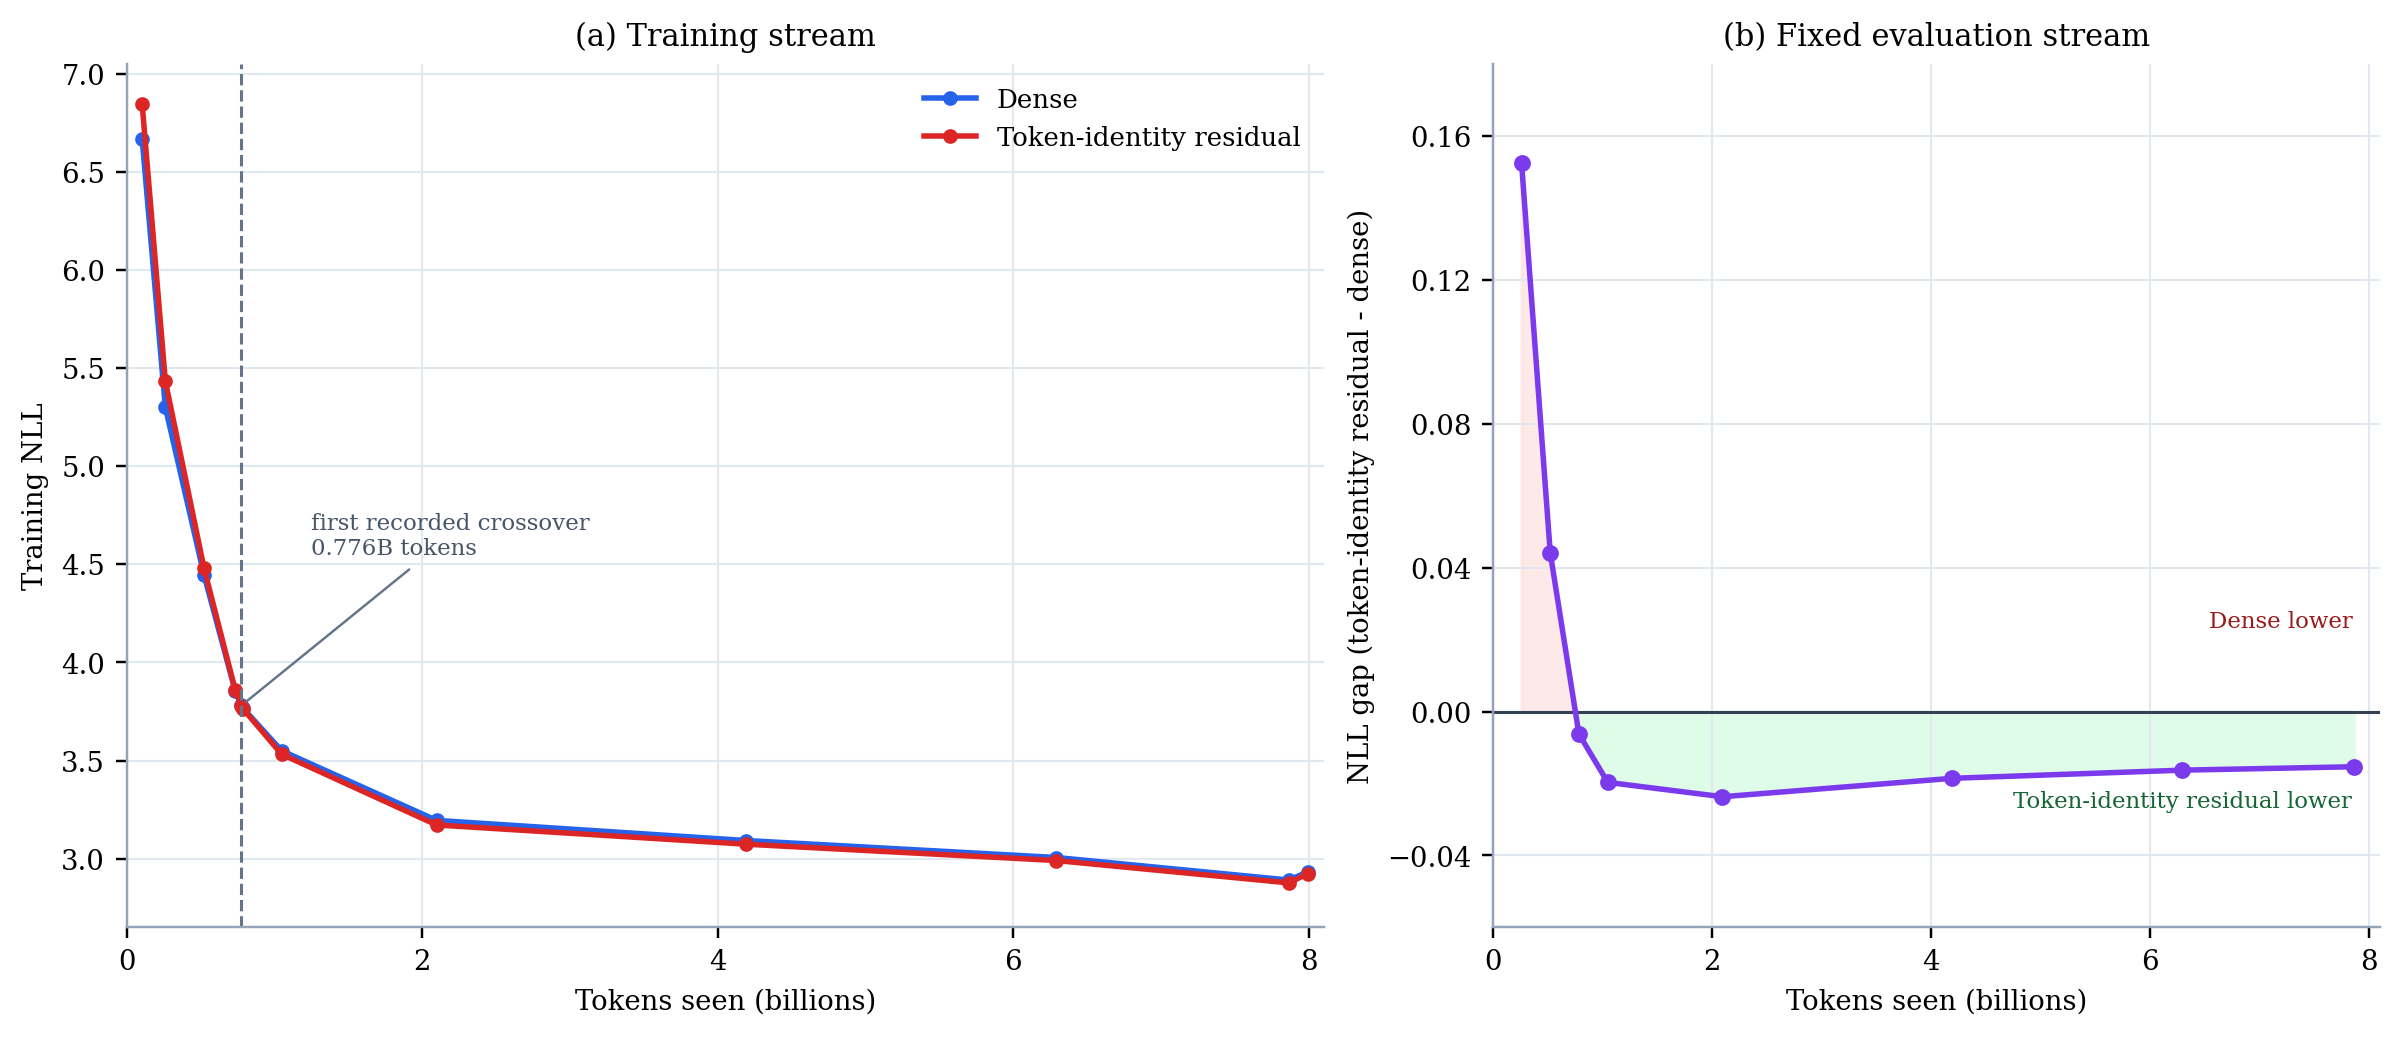
\includegraphics[width=0.86\textwidth]{fig_300m_loss_curves.png}
\caption{\textbf{Matched-token loss measurements.} \textbf{a}, Training NLL at recorded checkpoints. The token-identity residual model (red) begins behind dense (blue) and first crosses near 0.8 billion tokens. \textbf{b}, Token-identity residual minus dense NLL on the fixed FineWeb-Edu training-split evaluation stream; negative values favour token routing. Markers are recorded checkpoints and lines guide the eye. The evaluation stream is not held out, and each curve represents one seed.}
\label{fig:training}
\end{figure}

\begin{table}[t]
\centering
\small
\caption{\textbf{Matched-token loss trajectory.} All rows are training NLL except the explicitly labelled evaluation-stream row. Negative differences favour token routing. The evaluation stream is fixed across models but drawn from the FineWeb-Edu training split.}
\label{tab:trajectory}
\begin{tabular}{lrrrr}
\toprule
Measurement & Tokens & Dense & Token-routed & Difference \\
\midrule
Train & 105 million & \textbf{6.6698} & 6.8464 & $+0.1766$ \\
Train & 524 million & \textbf{4.4450} & 4.4796 & $+0.0346$ \\
Train & 1.05 billion & 3.5500 & \textbf{3.5324} & $-0.0176$ \\
Train & 2.10 billion & 3.1953 & \textbf{3.1720} & $-0.0233$ \\
Train & 4.19 billion & 3.0925 & \textbf{3.0738} & $-0.0187$ \\
Train & 6.29 billion & 3.0061 & \textbf{2.9906} & $-0.0154$ \\
Evaluation stream & 7.864 billion & 2.9482 & \textbf{2.9329} & $-0.0153$ \\
Train & 7.99 billion & 2.9324 & \textbf{2.9231} & $-0.0093$ \\
\bottomrule
\end{tabular}
\end{table}

The fixed vocabulary assignment does not mathematically ensure balanced corpus traffic. Observed final traffic was 0.2481, 0.2635, 0.2481 and 0.2403 across the four experts, with no inactive expert. On the same eight-B300 system and global batch, dense training reached approximately 0.95 million tokens per second and token routing 0.75 million tokens per second. The quality comparison is consequently matched by tokens, not by wall-clock time or compute.

\subsection*{Standard evaluations show near parity}

We evaluated the final step-7,629 checkpoints without task-specific fine-tuning using LM Evaluation Harness\cite{biderman2024reproducible}. The token-routed model is 0.46 percentage points below dense on ARC-Easy\cite{clark2018arc}, tied at displayed precision on PIQA\cite{bisk2020piqa}, 0.39 points above dense on HellaSwag\cite{zellers2019hellaswag}, and has 0.59 lower word perplexity on WikiText-2\cite{merity2017pointer} (Table~\ref{tab:benchmarks}). Each multiple-choice difference is smaller than one reported standard error. These tasks therefore support near parity, not task-level superiority.

\begin{table}[t]
\centering
\small
\caption{\textbf{Zero-shot evaluation of the final primary checkpoints.} Multiple-choice values are length-normalized accuracy in percent, reported as estimate $\pm$ standard error. WikiText-2 reports word perplexity (lower is better). Sample counts are 2,376, 1,838 and 10,042 for ARC-Easy, PIQA and HellaSwag, respectively.}
\label{tab:benchmarks}
\begin{tabular}{lrrrr}
\toprule
Model & ARC-Easy & PIQA & HellaSwag & WikiText-2 \\
\midrule
Dense & $\mathbf{49.07\pm1.03}$ & $\mathbf{63.49\pm1.12}$ & $33.67\pm0.47$ & 35.79 \\
Token-identity residual & $48.61\pm1.03$ & $\mathbf{63.49\pm1.12}$ & $\mathbf{34.06\pm0.47}$ & \textbf{35.20} \\
\bottomrule
\end{tabular}
\end{table}

\subsection*{Controls bound the interpretation}

Three internally matched panels provide controls at smaller scale (Table~\ref{tab:controls}). In the historical 1-billion-token panel, token-identity routing with a shared branch narrowly leads dense, whereas random routing and removing the shared branch are worse. In a separate 99.6-million-token diagnostic, an auxiliary-balanced learned top-2 router leads dense by 0.0119 evaluation NLL, while loss-free learned routing and fixed token-identity routing trail dense. Promoting the auxiliary router to a matched 1.0003-billion-token run reverses the short-budget ordering: dense leads by 0.0147 evaluation NLL and is approximately 5.2\% faster. These panels use the same o200k tokenizer family but different data ingestion and evaluation streams from the historical controls, so their absolute losses are not compared.

\begin{table}[t]
\centering
\scriptsize
\setlength{\tabcolsep}{4pt}
\caption{\textbf{Within-panel effects in smaller-scale controls.} Each value is the evaluation-NLL difference between a variant and the dense control from the same panel; negative values favour the variant. Panels use the same o200k tokenizer family, but the historical and contextual implementations use different data ingestion and evaluation streams.}
\label{tab:controls}
\begin{tabular}{llrr}
\toprule
Panel & Variant versus matched dense & Tokens & $\Delta$ evaluation NLL \\
\midrule
Historical fixed & Shared + balanced secondary & 1.0003B & $\mathbf{-0.0071}$ \\
& Shared + random top-2 & 1.0003B & $+0.0619$ \\
& Balanced secondary, no shared & 1.0003B & $+0.1435$ \\
\addlinespace
Contextual short & Learned top-2 + auxiliary balancing & 99.6M & $\mathbf{-0.0119}$ \\
& Learned top-2 + loss-free balancing & 99.6M & $+0.0286$ \\
& Fixed token-identity top-2 & 99.6M & $+0.0507$ \\
\addlinespace
Contextual full & Learned top-2 + auxiliary balancing & 1.0003B & $+0.0147$ \\
\bottomrule
\end{tabular}
\end{table}

\section*{Discussion}

These experiments isolate a modest effect: a fixed token identifier can select a useful residual parameter subspace while contextual computation remains shared. The result does not imply that token identifiers encode semantic expert classes. The primary assignments are modulo partitions up to a layer-specific permutation, and every active expert transforms the contextual hidden state. Stable token-conditioned access to parameters is sufficient to explain the observation.

The comparison also exposes practical trade-offs. Stored parameter count is matched, but active width differs slightly and the routed implementation is 21\% slower at the measured batch. Token routing therefore offers no demonstrated wall-clock or hardware-efficiency advantage. The auxiliary-balanced learned router leads dense at short budget but trails it in loss and throughput at the full budget. These single-seed controls do not establish that fixed routing is generally preferable.

The largest limitations are statistical and evaluative. Each architecture has one training seed, the loss-evaluation streams come from the training split, and the standard task panel is small. Accuracy gaps remain below one standard error. Replication across seeds, an independent held-out corpus, stronger out-of-distribution tasks and larger models are needed to assess robustness. A matched compute or wall-clock study would also be required to evaluate efficiency. The present evidence should consequently be read as a controlled architectural finding and a hypothesis for broader MoE studies.

Fixed routing removes one adaptive component and can simplify analysis, but it can also concentrate recurring token types in stable parameter subsets. We did not evaluate memorization, demographic performance, misuse or deployment safety. Any release of weights or application of the method should be accompanied by task-appropriate safety and data-governance evaluation.

\section*{Methods}

\subsection*{Transformer and residual experts}

Both primary models are decoder-only transformers with 18 layers, model dimension 1,024, 16 attention heads, four key--value heads, rotary positional embeddings, QK normalization, causal scaled dot-product attention and a maximum sequence length of 2,048. Feed-forward transformations use SwiGLU,
\begin{equation}
\operatorname{SwiGLU}(\mathbf{x})=
(\operatorname{SiLU}(\mathbf{x}\mathbf{W}_{\mathrm{gate}})\odot
\mathbf{x}\mathbf{W}_{\mathrm{up}})\mathbf{W}_{\mathrm{down}}.
\end{equation}
For model dimension $d$, shared width $d_s$, expert width $d_e$, $E$ stored experts and $k$ active experts, the routed layer stores $3d(d_s+Ed_e)$ weights and evaluates intermediate width $d_s+kd_e$. Tokens are grouped by their fixed assignments so that only selected routed experts are evaluated. The two selected outputs receive fixed weights 0.5 and 0.5 before multiplication by the learned routed gate.

\subsection*{Construction and verification of fixed routes}

Each layer uses a seeded permutation of four expert indices. Primary routes are obtained from the permuted token-ID residue. The secondary lookup is constructed once by iterating over token identifiers in ascending order and selecting, with lowest-index tie breaking, the least-used expert other than the primary. With a 32,000-entry vocabulary, every expert receives 8,000 primary identifiers. Checkpoint inspection verified that lookup buffers in all 18 layers reproduce this rule exactly. The construction uses no token counts or frequency table.

\subsection*{Primary training protocol}

Both primary models were trained on the same FineWeb-Edu token stream for 7,629 steps, corresponding to approximately 8 billion tokens. The tokenizer has 32,000 entries and the global batch contains 1,048,576 tokens (eight GPUs, batch 64 per GPU, sequence length 2,048). Training uses BF16 and AdamW with $\beta_1=0.9$, $\beta_2=0.95$, weight decay 0.1 and gradient clipping at 1.0. The learning rate uses a 5\% warm-up followed by cosine decay to 10\% of the peak. Residual output projections are initialized with standard deviation $0.02/\sqrt{2L}$ for $L$ layers\cite{radford2019language}. Apart from the MLP parameterization, run configuration, initialization seed, data order and token budget are matched.

Training NLL is read directly from the run metrics at matched steps. The fixed evaluation stream is identical for both models but sampled from the FineWeb-Edu training split; it is therefore a diagnostic of training progress, not held-out generalization. We report the last common evaluation point rather than an average of the final 50 training measurements. Throughput is the recorded steady-state training throughput on the same eight-NVIDIA-B300 system.

\subsection*{Control experiments}

The historical fixed-routing panel consists of seven approximately 100-million-parameter models trained for 1.0003 billion tokens on two NVIDIA B200 GPUs. It tests a dense residual MLP, a shared-only branch, a routed-only branch, random assignment and three deterministic top-2 labels. Inspection showed that the condition historically configured as frequency-aware had no populated frequency table and realized modulo-primary/cardinality-balanced-secondary assignment. Some named controls have equivalent primary assignments; differences among them are descriptive.

The contextual-router panels use the same o200k tokenizer family, a separate FineWeb-Edu memory-mapped shard, two NVIDIA RTX PRO 6000 Blackwell GPUs and a 98.2-million-parameter backbone. The learned router scores four residual experts from hidden states and selects two. The 99.6-million-token diagnostic compares dense, fixed token-identity routing, auxiliary-balanced learned routing and loss-free learned routing with the same seed, token order, batch and schedule. Only the auxiliary variant is promoted to a matched 1.0003-billion-token run against dense. Reported training NLL excludes the auxiliary term. The 1-billion-token runs have a 954-step budget, log training metrics every ten steps and evaluate every 750 steps; step 950 is therefore the last logged training point and step 750 the last evaluation checkpoint. The short runs analogously report training at step 95 and evaluation at step 75.

\subsection*{Standard evaluation}

Final step-7,629 checkpoints were exported to the same BF16 inference runtime. A five-prompt paired generation sanity test was completed before task evaluation. EleutherAI LM Evaluation Harness version 0.4.12 ran ARC-Easy, PIQA, HellaSwag and WikiText-2 with no sample limit, zero-shot prompts, automatic batching, a 2,048-token maximum context and seeds 1234 for Python, NumPy, PyTorch and few-shot sampling. We report \texttt{acc\_norm} for multiple-choice tasks and \texttt{word\_perplexity} for WikiText-2. The runtime used Transformers 4.57.6 and Datasets 5.0.0.

\subsection*{Statistics and reproducibility}

Training experiments use one seed per architecture; no confidence interval or hypothesis test is reported for loss. Multiple-choice standard errors are the task-level standard errors returned by the evaluation harness. Differences are shown at the precision supported by the measurements and are not converted into claims of statistical significance. Source metrics, configurations, route-verification tests, figure scripts and aggregate benchmark records accompany the supplementary code.

\subsection*{Use of generative artificial intelligence}

Generative artificial-intelligence tools were used as general-purpose assistants for language editing, consistency checks between the manuscript and author-provided CSV/JSON metric files, and figure and revision scripting. The authors designed and executed the experiments, reviewed and verified all experimental results, numerical values, scientific claims and final text, and take full responsibility for the manuscript.

\section*{Data availability}

FineWeb-Edu is publicly available under its applicable repository terms. The exact tokenizers, preprocessing instructions, run configurations and aggregate results needed to reproduce the reported analyses are included in the anonymized peer-review archive. The full checkpoint files and per-example evaluation logs are available to editors and reviewers on request and will be deposited in a persistent public repository upon publication.

\section*{Code availability}

An anonymized source archive containing the PyTorch implementation, fixed and learned routing variants, route tests, training entry points and analysis scripts accompanies the submission. A public, versioned repository and archival release will be provided upon publication.

\section*{Author contributions}

Author names and contribution details are withheld from this double-anonymized manuscript and are supplied in the cover letter.

\section*{Competing interests}

A complete competing-interests declaration is supplied in the cover letter for double-anonymized review.

\bibliographystyle{unsrtnat}
\bibliography{nature_references}

\end{document}
